\documentclass[tikz, border=10pt]{standalone}
\usepackage{pgfplots}
\pgfplotsset{compat=1.18}

\begin{document}
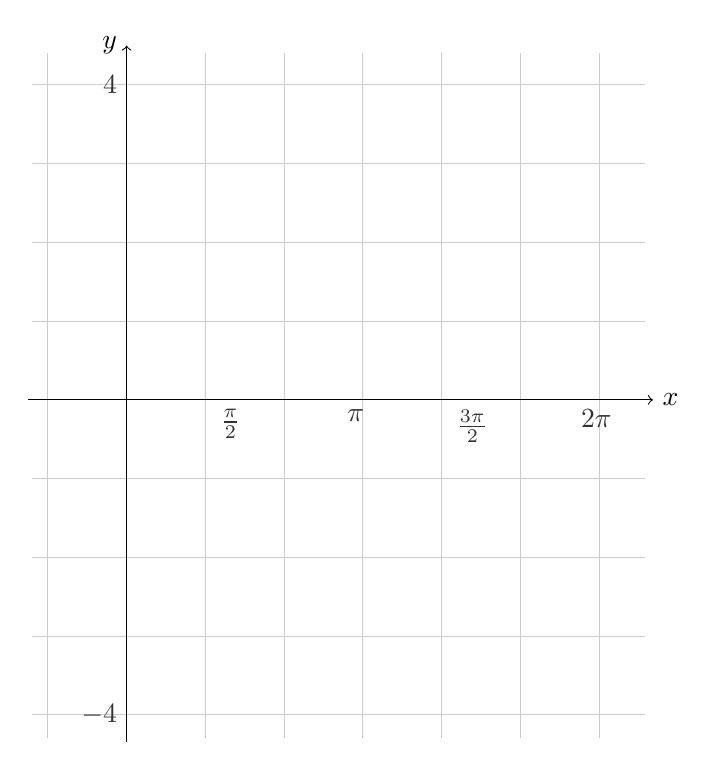
\begin{tikzpicture}
    \draw[thin, color=black!20] (-1.2,-4.3) grid (2*pi+0.3,4.4);
    \draw[->] (-1.25,0) -- (2*pi+0.4,0) node[right] {$x$};
    \draw[->] (0,-4.35) -- (0,4.5) node[left] {$y$};
    % several curves for the problem
    \draw[color=black!80!red] plot[samples=400, id=travelingWave1, domain=0:2*pi] function{4*sin(2*x)}; %node[right] {$\sin(x)$};
    \draw[color=black!50] plot[samples=400, id=travelingWave2, domain=0:2*pi] function{4*0.84*sin(2*x)}; %node[right] {$\sin(x)$};
    \draw[color=black!50] plot[samples=400, id=travelingWave3, domain=0:2*pi] function{4*0.73*sin(2*x)}; %node[right] {$\sin(x)$};
    \draw[color=black!50] plot[samples=400, id=travelingWave4, domain=0:2*pi] function{4*0.5*sin(2*x)}; %node[right] {$\sin(x)$};
    %points
    \draw[color=black!80] (0,-4) node[left] {$-4$};
    \draw[color=black!80] (0,4) node[left] {$4$};
    \draw[color=black!80] (pi/2,0) node[anchor=north east] {$\frac{\pi}{2}$};
    \draw[color=black!80] (pi,0) node[anchor=north east] {$\pi$};
    \draw[color=black!80] (3*pi/2,0) node[anchor=north east] {$\frac{3\pi}{2}$};
    \draw[color=black!80] (2*pi,0) node[anchor=north east] {$2\pi$};
\end{tikzpicture}
\end{document}
